\section{George Green}
Der Namensgeber f�r die Greensche Funktion ist George Green. Er war ein britischer Physiker und Mathematiker. Geboren wurde er 1793 in der N�he von Nottingham. Sein Vater betrieb eine M�hle und George Green arbeitete ebenfalls als M�ller. Nach dem Tod seines Vaters f�hrte er den M�hlenbetrieb fort. Bemerkenswert ist, dass Green nur etwa zwei Jahre in die Schule ging. Mathematische und Physikalische Grundlagen brachte er sich selber bei. Der Ort an dem er lehrte war seine M�hle. Da nie ein Portrait von ihm angefertigt wurde, gibt es kein Bild von ihm. Darum wird anstatt seinem Konterfei jeweils eine Windm�hle verwendet um ihn darzustellen. Die Windm�hle gibt es �brigens immer noch. Green ver�ffentliche mit etwa dreissig Jahren seine erste Arbeit. Diese wurde kaum beachtet, ausser von einem adligen Mathematik Namens Sir Edward Bromhead. Er ermutigte Green, im Alter von vierzig Jahren in Cambridge zu studieren. Interessant zu wissen ist dazu, dass dort zu dieser Zeit die Theorien von Laplace und Fourier noch nicht gelehrt wurde. Green hatte sich jedoch durch diese Theorie gelesen und sogar noch einige Erweiterungen hinzugef�gt. Vier Jahre nachdem er graduierte und kurz vor seinem Internationalen Durchbruch stand, starb er 1841 jedoch an einer schweren Grippe. Dadurch geriet seine Arbeit f�r einige Zeit in Vergessenheit.

George Green ist besonders bekannt f�r das Greensche Theorem und die Greensche Funktion. Er besch�ftigte mit der L�sung von partiellen Differentialgleichungen und stellte damit unter anderem mathematische Hilfsmittel bereit, die sogar in der Quantenfeldtheorie im 20. Jahrhundert von Bedeutung waren.\cite{wiki:green}

Neben vielen anderen Pers�nlichkeiten wie Maxwell, Dirac oder Newton ist er in der Westminster Abbey in London mit einer Gedenktafel verewigt\cite{wiki:westminster}. Der Grund, warum George Green nicht so popul�r ist wie Gauss oder Maxwell, liegt wahrscheinlich darin, dass von seiner Zeit, als er in seiner M�hle gearbeitet hat, wenig  bekannt ist. Auch war er nur f�r sehr kurze Zeit in Cambridge t�tig. Trotzdem war es an dieser Stelle das Ziel einen so einzigartigen Wissenschaftler, der seiner Zeit um einiges voraus war, mehr als nur zu erw�hnen.

	\begin{figure}[htb]                     \centering 
	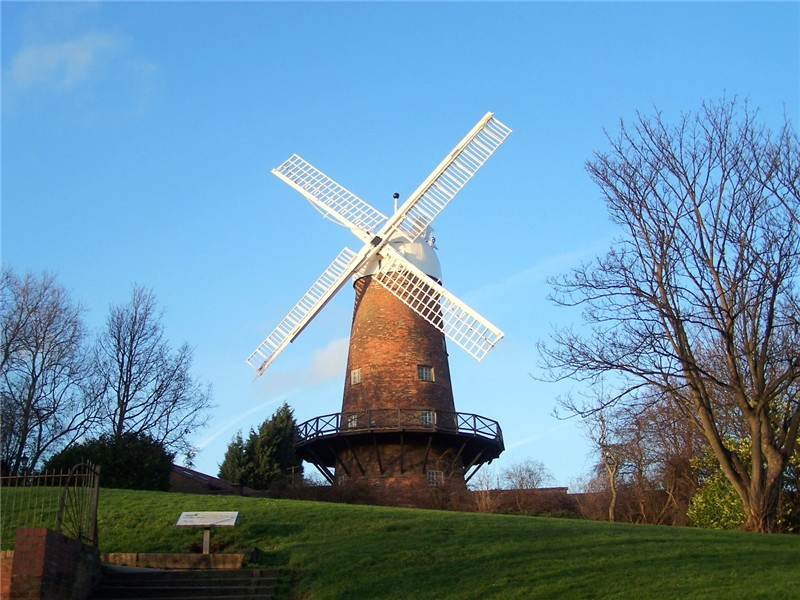
\includegraphics[width=8cm]{images/greens_windmill} 
	\caption{Windm�hle, in der Green f�r lange Zeit gearbeitet hat} 
	\label{fig:abb1} 
	\end{figure} 